\subsection{Assimetria}

Assimetria é o grau de desvio ou afastamento da simetria de uma distribuição.

Quando a curva é simétrica, a média, a mediana e a moda coincidem,
num mesmo ponto, de ordenada máxima, havendo um perfeito equilíbrio na distribuição. Quando o equilíbrio não acontece, isto é, a média, a mediana e a moda recaem em pontos diferentes da distribuição esta será assimétrica; enviesada a direita ou esquerda.

\begin{align*}
\text{Simetria} &\Rightarrow\text{Assimetria}\, (S)=0\\
&Mo=Md=\bar{c}
\end{align*}
\begin{figure}[H]
    \centering
    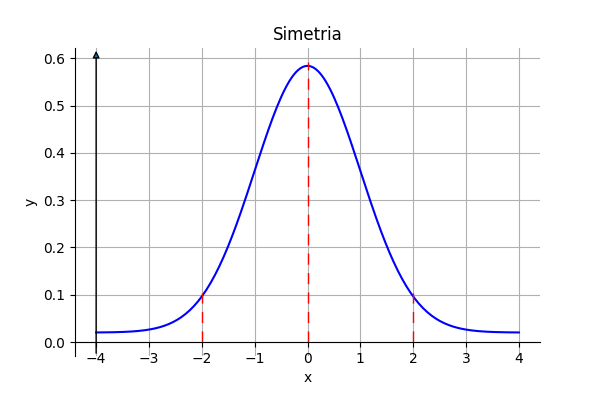
\includegraphics[width=0.8\linewidth]{simetria.png}
    \caption{$Mo=Md=\bar{x}$}
\end{figure}

Distribuição assimétrica Negativa ou enviesada a esquerda - quando os valores se concentram na extremidade superior da escala e se distribuem gradativamente em direção à extremidade inferior.

Distribuição assimétrica Positiva ou enviesada a direita quando os
valores se concentram na extremidade inferior da escala e se distribuem gradativamente em direção à extremidade superior

\begin{align*}
\text{Simetria} &\Rightarrow\text{Assimetria}\, (S)=0\\
&Mo=Md=\bar{c}
\end{align*}

\begin{figure}[H]
    \centering
    
\includegraphics[width=0.8\linewidth]{./figs/assimetria_esquerda.png}
    \caption{$Mo < Md < \bar{x} $}
\end{figure}

\begin{figure}[H]
    \centering
    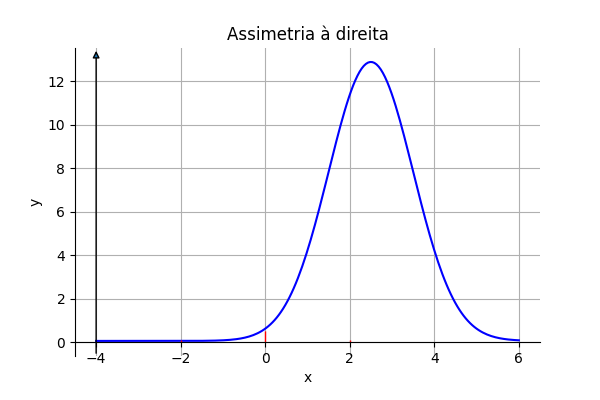
\includegraphics[width=0.8\linewidth]{./Figs/assimetria_direita.png}
    \caption{$Mo > Md >\bar{x} $}
\end{figure}

Cálculo aa Assimetria: critério de Bowley
\[
 Q3 - Md \neq Md - Q1
 \]
 \[ 
 S=\frac{Q3+Q1-2Md}{Q3-Q1}\qquad\text{assimetria relativa; $-1\leq S\leq 1$}
  \]
Será Positivo a medida que o terceiro quartil se afasta da mediana, enquanto o primeiro quartil se aproxima da mesma, tendo como limite: $Q1 = Q2$, quando a assimetria assume o valor máximo positivo: $(S = 1)$.
 \[ 
 S=\frac{Q3-Q1}{Q3-Q1}=1
  \]
  Será Negativo a medida que o primeiro quartil afasta-se da mediana, enquanto o terceiro quartil aproxima-se da mesma, dando como limite: \[Q3 = Q2\] quando a assimetria assume valor máximo negativo:
\[ 
 S=\frac{-Q3-Q1}{Q3-Q1}=-1
\]

Critério de Kelley - Para corrigir parte do inconveniente de se desprezar 50\% das ocorrências (Critério de Bowley), Kelley aconselha o uso dos “Centis” eqüidistantes da mediana, tais como C10 e C90, para cálculo assimetria.
 \[ 
 S=\frac{C_{90}+C_{10}-2Md}{C_{90}-C_{10}}\qquad\text{cujos limites variam também de $[-1,+1]$}
  \]
  Coeficiente de Assimetria de Pearson -- Á medida que a distribuição deixa de ser simétrica, a média, a mediana e a moda vão se afastando, aumentando cada vez mais a diferença entre elas
  \[
    \text{Coeficiente de Assimetria de Pearson (1º)}\;S_{k1}=\frac{(\bar{x}-Mo)}{s}
  \]
  \[
    \text{Coeficiente de Assimetria de Pearson (2º)}\;S_{k2} =
    \frac{3(\bar{x}-Me)}{s}
  \]
  \subsection{Curtose}
  É o grau de achatamento de uma distribuição, em relação à distribuição normal. A curtose pode ser de três tipos:
\begin{itemize}[label=\diamondsuit]
    \item Mesocúrtica - quando a distribuição é normal.
    \item Leptocúrtica - quando a distribuição é mais pontiaguda que a normal
    \item Platicúrtica - quando a distribuição é mais achatada que a normal.
\end{itemize}

\begin{figure}[H]
    \centering
    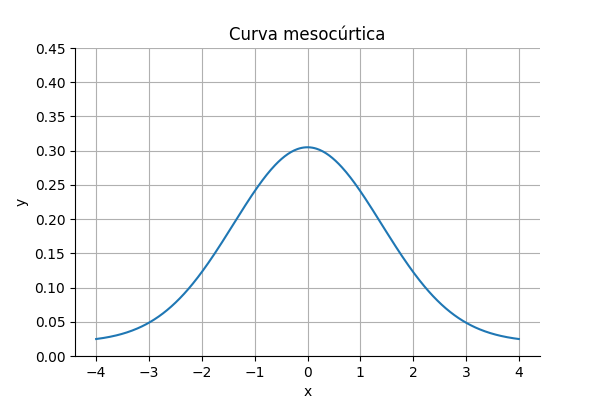
\includegraphics[width=0.8\linewidth]{./Figs/mesocurtica.png}
    \caption{}
\end{figure}

\begin{figure}[H]
    \centering
    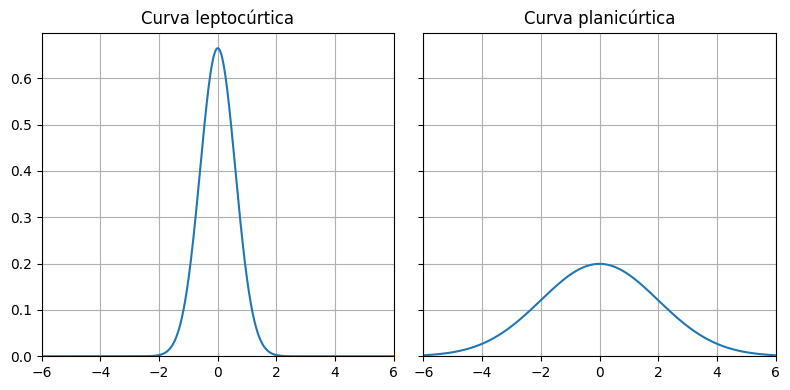
\includegraphics[width=0.8\linewidth]{./Figs/fig_lepto_plani.png}
    \caption{}
\end{figure}

A curtose é uma medida de forma que descreve o grau de achatamento ou concentração de uma distribuição em torno da média.

\subsubsection{Curtose pelo Método dos Momentos (Fisher)}

Sejam $\mu_4$ o momento central de quarta ordem e $\sigma$ o desvio padrão populacional. Define-se o coeficiente de curtose como:

\[
\beta_2 = \frac{\mu_4}{\sigma^4}
\]

O coeficiente de curtose de Fisher (excesso de curtose) é dado por:

\[
\gamma_2 = \beta_2 - 3
\]

Para a distribuição normal:

\[
\gamma_2 = 0
\]

Classificação:

\begin{itemize}
    \item $\gamma_2 = 0$ : Mesocúrtica (mesmo achatamento da normal)
    \item $\gamma_2 > 0$ : Leptocúrtica (mais concentrada no centro e com caudas mais pesadas)
    \item $\gamma_2 < 0$ : Platicúrtica (mais achatada que a normal)
\end{itemize}

\subsubsection{Curtose Percentílica (Coeficiente de Kelley)}

Uma medida alternativa e mais robusta baseia-se em quantis.

Sejam:

\begin{itemize}
    \item $Q_1$ = primeiro quartil (25\%)
    \item $Q_3$ = terceiro quartil (75\%)
    \item $P_{10}$ = percentil 10
    \item $P_{90}$ = percentil 90
\end{itemize}

Define-se inicialmente a semi-amplitude interquartílica:

\[
D_q = \frac{Q_3 - Q_1}{2}
\]

O coeficiente de curtose percentílica é dado por:

\[
C = \frac{Q_3 - Q_1}{2(P_{90} - P_{10})}
\]

Para a distribuição normal padrão, obtém-se aproximadamente:

\[
C_{\text{normal}} \approx 0,263
\]

Classificação segundo Kelley:

\begin{itemize}
    \item $C = 0{,}263$ : Mesocúrtica
    \item $C < 0{,}263$ : Leptocúrtica
    \item $C > 0{,}263$ : Platicúrtica
\end{itemize}

\subsubsection{Observação}

O coeficiente de Fisher mede curtose com base nos momentos da distribuição, sendo sensível a valores extremos.

O coeficiente de Kelley utiliza quantis, sendo mais robusto e frequentemente empregado em Estatística Descritiva introdutória.